
%(BEGIN_QUESTION)
% Copyright 2014, Tony R. Kuphaldt, released under the Creative Commons Attribution License (v 1.0)
% This means you may do almost anything with this work of mine, so long as you give me proper credit

Determine the magnitude and phase shift of the output voltage ($V_{out}$) with reference to the source voltage (0$^{o}$) for each of the two switch positions, assuming the source frequency is such that $X_C = R$:

$$\includegraphics[width=15.5cm]{i00845x01.eps}$$

Note: you should be able to do the phase shift calculation mentally, without the aid of a calculating device!  It is also possible to determine the output voltage magnitude without the aid of a calculating device if you are familiar enough with the values of common trignometric functions.

\underbar{file i00845}
%(END_QUESTION)





%(BEGIN_ANSWER)

Switch left: $\theta$ = $-45^{o}$ ($V_{out}$ lagging behind the source voltage)

\vskip 10pt

Switch right: $\theta$ = $+45^{o}$ ($V_{out}$ leading ahead of the source voltage)

\vskip 10pt

In both positions, the output voltage magnitude will be $\sqrt{2} \over 2$ that of the input voltage, or $0.707 \times V_{signal}$, because both the sine and the cosine of 45$^{o}$ is $\sqrt{2} \over 2$.  

%(END_ANSWER)





%(BEGIN_NOTES)


%INDEX% Electronics review: AC reactance and impedance
%INDEX% Electronics review: series-parallel AC circuits

%(END_NOTES)

